\chapter{Metodología}\label{ch:chapter_3}

En este proyecto se utilizaron metodologías ágiles para mejorar la calidad y eficiencia del desarrollo de software.
La programación extrema facilitó ciclos de desarrollo cortos y una comunicación fluida con la directora del TFG,
mientras que el desarrollo dirigido por pruebas garantizó un diseño bien probado.
La metodología iterativa incremental permitió evaluar y ajustar avances rápidamente, y la gestión visual de procesos con
Kanban mejoró la visibilidad y gestión del flujo de trabajo.

\section{Metodologías ágiles}

En este proyecto se utilizaron las siguientes metodologías enmarcadas dentro de las metodologías ágiles.
La \textit{programación extrema} introdujo los ciclos de desarrollo cortos y frecuentes, así como la comunicación
fluida con los miembros del equipo, en este caso mi directora de TFG.
El \textit{desarrollo dirigido por pruebas} ayudó a obtener un diseño óptimo y bien testeado, mientras que la
\textit{metodología iterativa incremental} permitió evaluar los avances en pequeños pasos, permitiendo tomar
decisiones rápidamente cuando fue necesario.

\subsection{Programación extrema}

La Programación Extrema o \textit{extreme programming} (XP) es una metodología ágil de desarrollo de software que se
enfoca en mejorar la calidad del software y la capacidad de respuesta a las necesidades cambiantes del cliente.
Introducida por Kent Beck en el libro \textit{Extreme Programming Explained: Embrace Change}~\cite{book_beck_1999},
XP promueve la colaboración intensa entre los desarrolladores y los clientes, ciclos de desarrollo cortos y frecuentes,
y la entrega continua de pequeñas mejoras.

\subsection{Desarrollo dirigido por pruebas}

El desarrollo dirigido por pruebas o \textit{test driven development} (TDD) es una práctica de desarrollo de software.
Este enfoque fue popularizado por Kent Beck, uno de los pioneros de las metodologías ágiles, en su libro
\textit{Test Driven Development: By Example}~\cite{book_beck_2003}.
TDD se basa en ciclos cortos de desarrollo donde se escribe una prueba, se implementa el código necesario para pasar la
prueba y luego se reescribe el código para mejorar su estructura sin cambiar su comportamiento.

\subsection{Iterativo incremental}\label{subsec:iterativo_incremental}

El enfoque iterativo incremental es una metodología utilizada en el desarrollo de software que combina dos modelos:
el iterativo y el incremental.
Esta metodología es popular en el desarrollo ágil y se centra en desarrollar un sistema a través de ciclos repetidos
(iteraciones) y en la construcción gradual de funcionalidad (incrementos).

El término ``iterativo'' se refiere a la repetición de un conjunto de actividades a lo largo del ciclo de vida del
desarrollo del software.
En cada iteración, se planea, desarrolla y evalúa una parte del sistema.

El término ``incremental'' se refiere a la construcción del sistema mediante adiciones sucesivas de componentes y
funcionalidades.
Cada incremento agrega una parte funcional del sistema hasta que el producto está completo.
\section{Gestión visual de procesos}

La gestión visual de procesos o \textit{kanban} es un método de gestión de proyectos que se originó en la industria
manufacturera japonesa, específicamente en Toyota, como una forma de mejorar la eficiencia de la producción y que se
encuentra fuertemente implantado dentro de la industria del desarrollo de software~\cite{book_anderson_2010}.

El término significa ``tarjeta visual'' en japonés, y el método se basa en el uso de tarjetas visuales para
representar tareas en un tablero, permitiendo a los miembros del equipo ver el estado del progreso del trabajo de un
simple vistazo.

\begin{figure}[ht]
    \begin{center}
        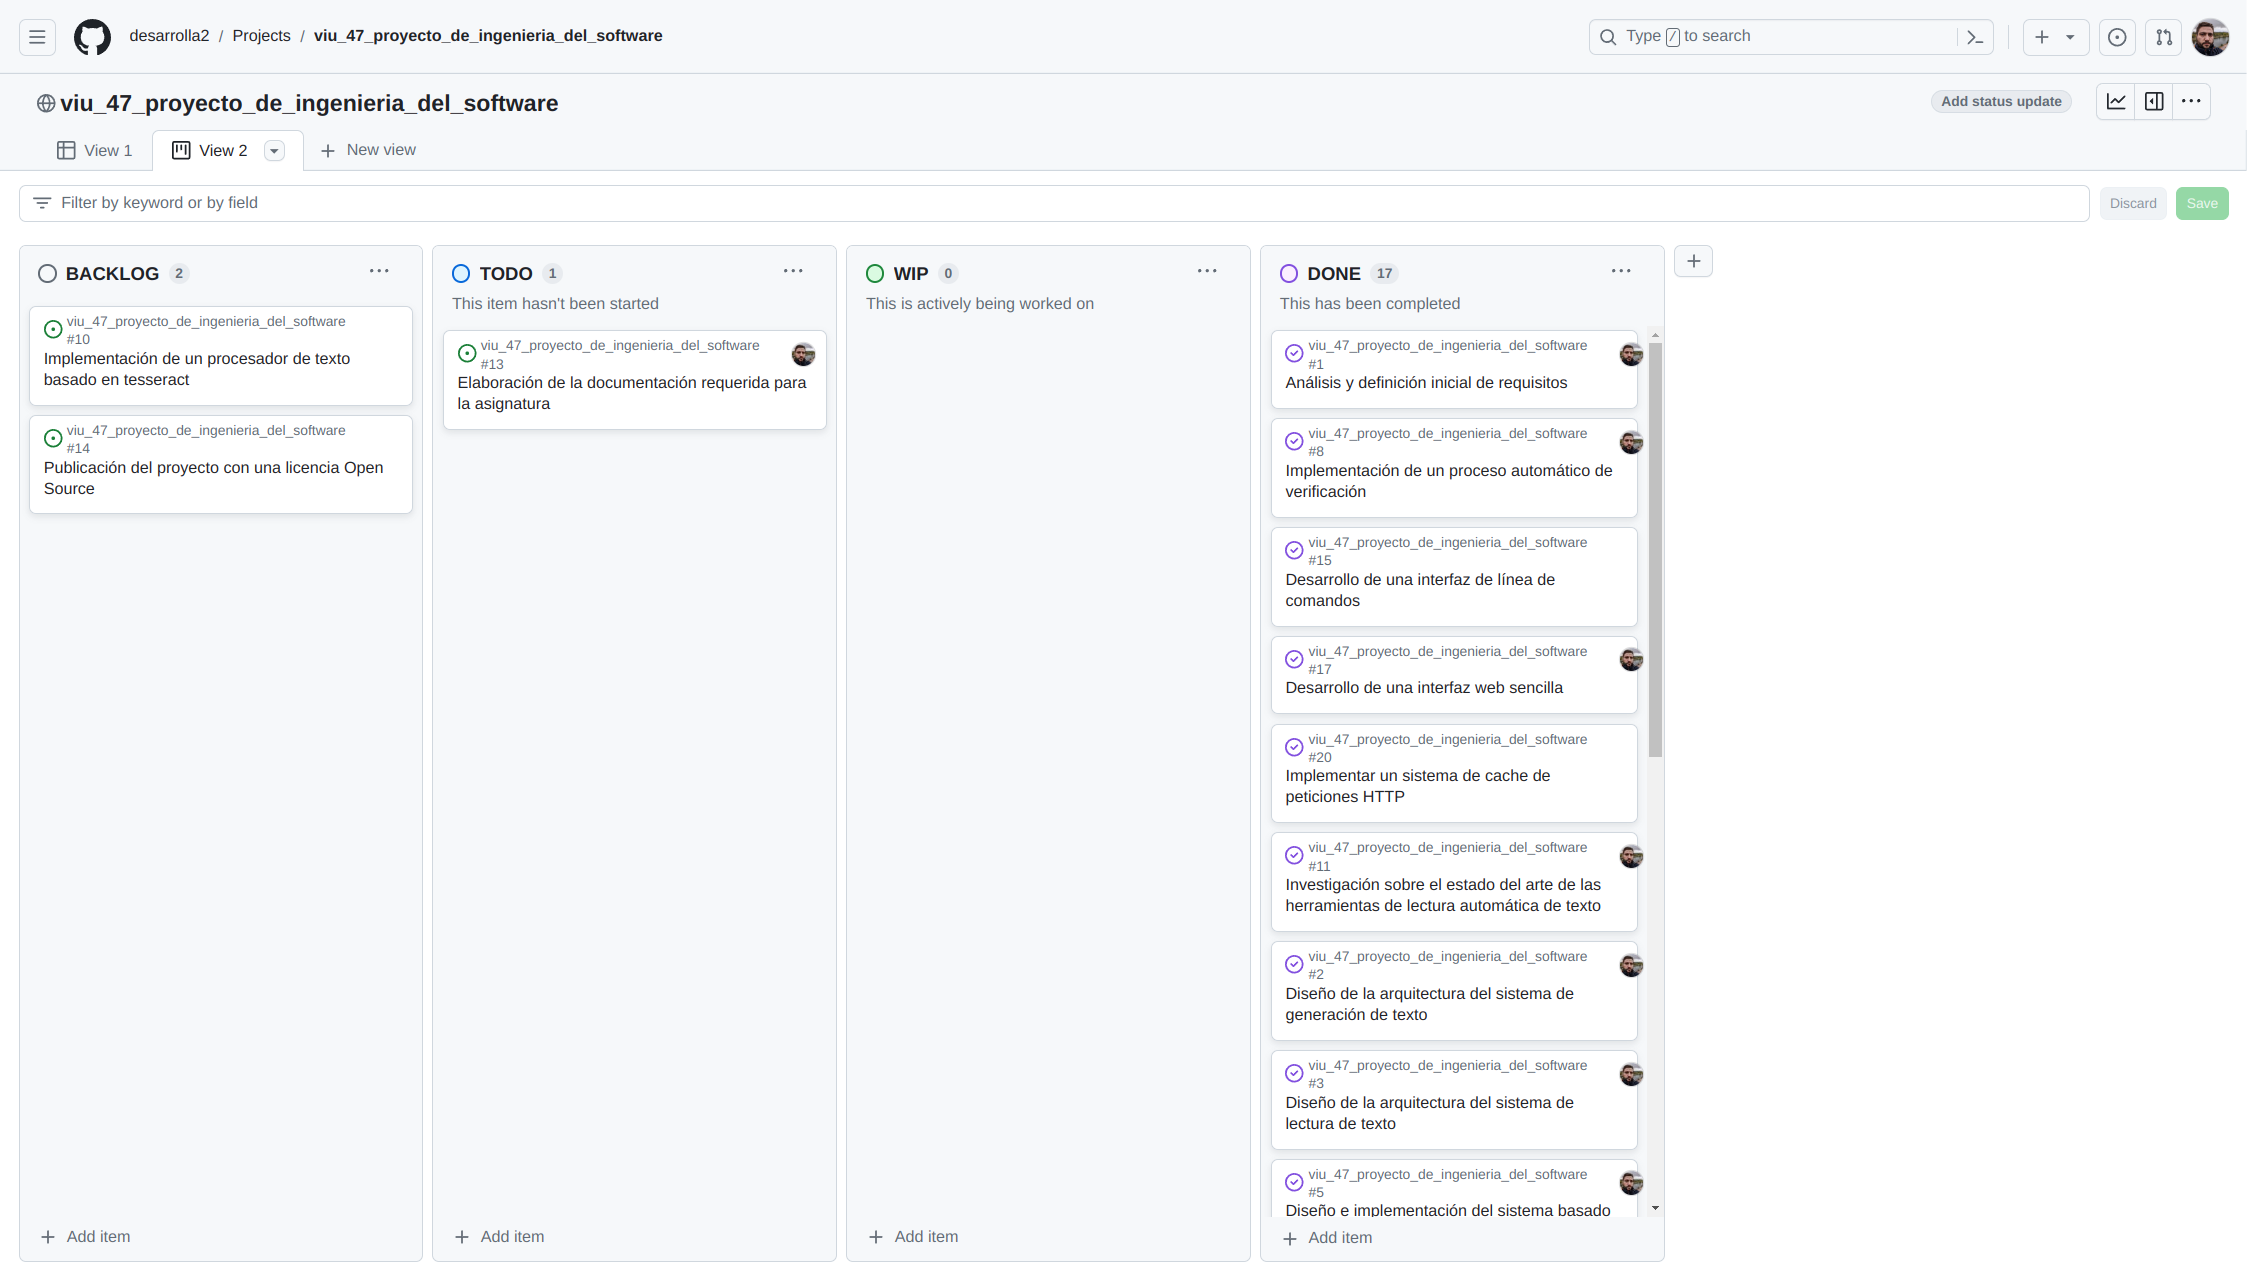
\includegraphics[width=\textwidth]{./chapter/3/images/chapter_3.kanban}
        \caption{Captura del tablero kanban del proyecto}
        \label{fig:chapter_3.kanban}
    \end{center}
\end{figure}

\textit{Kanban} promueve la mejora continua, la flexibilidad y la eficiencia, ayudando a los equipos a gestionar el
flujo de trabajo y a identificar cuellos de botella rápidamente.

En la figura~\ref{fig:chapter_3.kanban} puede una captura de cómo hemos usado \textit{Kanban} para la gestión de las
tareas, teniendo en todo momento una visión completa del estado de avance de cada \textit{iteración}.

Al inicio del proyecto las tareas fueron definidas e incluidas en la columna \textbf{backlog}.
Durante el desarrollo del proyecto, si una nueva tarea era identificada, se incluía dentro de esta columna.

Al inicio de cada iteración, se realiza una planificación donde algunas tareas son incluidas dentro de la iteración
y las tareas son desplazadas a la columna \textbf{todo}.
Estas tareas deben encontrarse correctamente definidas y claras y el volumen total del trabajo debe estar adecuado a
la capacidad del equipo y del tiempo disponible en la iteración.

Durante la iteración las tareas se van desplazando a la columna \textbf{WIP} o \textit{work in progress} para
indicar que están siendo realizadas en este momento y finalmente a la columna \textbf{DONE}, una vez que son
completadas.

Al terminar cada iteración, todo el trabajo no completado, se desplaza de nuevo al \textit{backlog}.
Se realizan dos ceremonias, en una denominada \textit{demo} o demostración se realiza una demostración del trabajo
realizado, mientras que en la segunda, la \textit{retrospectiva} se realiza un análisis de los puntos fuertes y
puntos débiles del proceso de trabajo, con el objetivo de mitigar cualquier problema que pudiera surgir.

A modo de ejemplo añado los videos de ejemplo de una planificación~\cite{url_viu_47_proyecto_ingenieria_sprint_6_plan},
una demo~\cite{url_viu_47_proyecto_ingenieria_sprint_6_demo} y una
retrospectiva~\cite{url_viu_47_proyecto_ingenieria_sprint_6_retrospectiva} de la asignatura Proyecto de Ingeniería del
Software.
